\documentclass[border=4pt]{standalone}
\usepackage{tikz}
\usetikzlibrary{arrows.meta,positioning,shapes.geometric}
\begin{document}
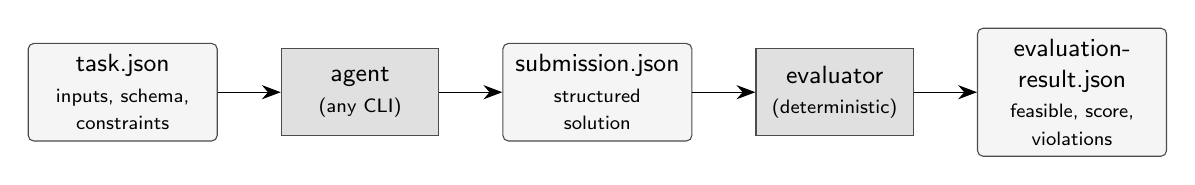
\begin{tikzpicture}[
  font=\sffamily\small,
  artifact/.style={rectangle, rounded corners=2pt, draw=black!70, fill=black!4,
                   minimum height=11mm, minimum width=24mm, align=center, inner sep=4pt},
  actor/.style={rectangle, draw=black!70, fill=black!12, minimum height=11mm,
                minimum width=20mm, align=center, inner sep=4pt},
  >={Stealth[length=2.4mm]}, node distance=8mm]
  \node[artifact] (task) {task.json\\\scriptsize inputs, schema,\\[-1pt]\scriptsize constraints};
  \node[actor, right=of task] (agent) {agent\\\scriptsize (any CLI)};
  \node[artifact, right=of agent] (sub) {submission.json\\\scriptsize structured\\[-1pt]\scriptsize solution};
  \node[actor, right=of sub] (eval) {evaluator\\\scriptsize (deterministic)};
  \node[artifact, right=of eval] (res) {evaluation-\\result.json\\\scriptsize feasible, score,\\[-1pt]\scriptsize violations};
  \draw[->] (task) -- (agent);
  \draw[->] (agent) -- (sub);
  \draw[->] (sub) -- (eval);
  \draw[->] (eval) -- (res);
\end{tikzpicture}
\end{document}
